\section{Erstes Modell}

Das Jupyter-Notebook zu diesem Kapitel kann über \aka{https://github.com/klawr/deepmech/blob/master/reports/srp/notebooks/5-first_model.ipynb} eingesehen werden.

\subsection{Projektstruktur}

Die Projektstruktur ist ein wichtiger Teil, um Modelle effizient zu testen und sie gegen andere Modelle zu evaluieren, um das beste Modell zu bestimmen.
\name{deepmech} ist unter Verwendung einer modifizierten Version der Cookiecutter Data Science \cite{drivendata2019} Struktur aufgebaut. Sie kann unter \url{klawr.github.io/deepmech} eingesehen werden.

Der Stammordner enthält Dateien wie die Lizenz des gesamten Projekts.
Das Projekt ist unter der MIT-Lizenz lizenziert, die jedem Menschen die Möglichkeit gibt, es für den privaten und kommerziellen Gebrauch zu verändern, zu verteilen oder zu nutzen, aber unter Ausschluss jeglicher Haftung oder Gewährleistung meinerseits.
Im Stammordner befindet sich eine weitere Datei \name{requirements.txt}, die Teil des Installationsprozesses ist und es erlaubt, den gesamten in diesem Projekt behandelten Code zu replizieren.

Die "Cookiecutter Data Science"-Struktur ermöglicht eine klare Verteilung der Daten in Rohdaten (die nie angefasst werden dürfen), Zwischendaten (das sind die Rohdaten, die aber in irgendeiner Weise modifiziert, ergänzt oder verändert werden) und verarbeiteten Daten (die über einen Trainingsalgorithmus in das Modell eingespeist werden sollen).
Diese Daten werden im Verzeichnis \name{data} gespeichert.

Logs werden während des Trainings mit \name{TensorBoard}\footnote{TensorBoard ist das Visualisierungs-Toolkit von \name{TensorFlow}. Die mit \name{TensorBoard} erzeugten Visualisierungen werden später gezeigt.} erstellt.
Diese Protokolle werden durch einen Zeitstempel des jeweiligen Trainingslaufs unterschieden und befinden sich im Verzeichnis \name{logs}.

Die derzeit verwendeten Modelle befinden sich im Verzeichnis \name{models}.
Die Modelle in diesem Verzeichnis können sich in verschiedenen Phasen des Projektes ändern, so dass die jeweiligen Berichte ihre eigenen Modellverzeichnisse haben, um die Zwischenmodelle zu speichern.

Im \name{reports} Verzeichnis befindet sich jeweils einem Ordner für jedes in diesem Projekt erstellten Berichten, einschließlich dieses Artikels\footnote{Versehen mit dem Namen \name{srp}, für Student Research Project}.
Der \name{notebook}-Ordner in diesem Bericht enthält die Jupyter-Notebooks \cite{Jupyter2019}, die in den unterschiedlichen Kapiteln genutzt wurden.
Die Modelle werden ebenfalls innerhalb von \name{Jupyter} Notebooks trainiert. 
Jupyter notebooks sind interaktive Python-Code-Editoren, die eine einfache Möglichkeit bieten, effizient Code zu schreiben, zu testen und (mittels Markdown) zu kommentieren.
Alle Notebooks mit entsprechendem Code befinden sich im Verzeichnis \name{notebooks} im Stammverzeichnis dieses Projekts\footnote{\aka{https://github.com/klawr/deepmech/tree/master/reports/srp/notebooks/}}.
Das jeweilige Verzeichnis der Ausarbeitungen enthält auch den verwendeten Code, die trainierten Modelle, Bilder und die für die Erstellung dieses Berichts erstellten Dokumente.

\name{src} enthält den gesamten Code (mit Ausnahme der in den Berichten verwendeten Demos), der bei der Entwicklung und dem Training der Modelle verwendet wurde. Sie reichen von Skripten, die geeignete Umgebungen zum Trainieren der Modelle schaffen, bis hin zur Datengenerierung und -augmentierung.

\subsection{Laden von Daten}

Bevor das Training des Modells beginnen kann, müssen die Daten geladen werden.
Wie erwähnt werden die Daten in diesem Projekt im Verzeichnis \name{raw} des Verzeichnisses \name{data} gespeichert.
Es ist eine gute Praxis, nie direkt mit den Rohdaten zu arbeiten, daher enthält der Beginn jeder Trainingseinheit eine Vorbereitungsphase, in der die Rohdaten in das \name{processed} Datenverzeichnis kopiert werden (eventuell mit Erweiterungen oder Änderungen in Zwischenschritten).

Demnach beginnt das Training eines Modells in diesem Projekt stets mit folgendem Code:

\begin{lstlisting}
    from os.path import join
    
    raw = join('data', 'raw')
    interim = join('data', 'interim')
    processed = join('data', 'processed')
        
    from src.utils import reset_and_distribute_data
        
    reset_and_distribute_data(raw, processed, [400, 0, 100])
\end{lstlisting}

Für das erste Modell reichen die Rohdaten selbst aus; daher werden sie einfach mit einer vordefinierten Funktion \code{reset\_and\_distribute\_data} aus \code{src/utils.py} in das Verzeichnis der verarbeiteten Daten kopiert.
Der dritte Parameter von \code{reset\_and\_distribute\_data} ist ein Array mit drei Zahlen, die die Verteilung der Trainings-, Validierungs- und Testdaten beschreiben.
In diesem Beispiel werden die Validierungsdaten weggelassen, da keine Anpassungen an den Hyperparametern vorgenommen werden.

\begin{lstlisting}
    from tensorflow.keras.preprocessing.image import ImageDataGenerator
    
    def create_generator(data_dir, batch_size):
        datagen = ImageDataGenerator(rescale=1./255)
        full_path = join(processed, data_dir)
        return datagen.flow_from_directory(
            full_path,
            target_size=(32, 32),
            batch_size=batch_size,
            class_mode='binary')
    
    train_generator = create_generator('train', 20)
    test_generator = create_generator('test', 10)
\end{lstlisting}

Nachdem die entsprechenden Daten auf die verschiedenen Verzeichnisse verteilt sind, wird der \code{ImageDataGenerator}\footnote{\aka{https://keras.io/preprocessing/image/}} verwendet, um dem Modell zu ermöglichen, die Daten später während des Trainingsprozesses zu laden.
Die Generatoren definieren auch die Größe des geladenen Bildes, die auf 32 Pixel Breite und 32 Pixel Höhe\footnote{Die Größe der Bilder wird manuell bestimmt, indem man davon ausgeht, dass der Algorithmus, solange ein Mensch in der Lage ist, die charakteristischen Merkmale des Bildes zu erkennen, diese erlernen kann.} (im Gegensatz zur ursprünglichen Bildgröße von 512x512) und eine Batch-Größe\footnote{Die Batch-Größe ist die Anzahl der Bilder, die zwischen jedem Backpropagationszyklus verwendet werden.
Wenn die Batch-Größe mit der Datensatzgröße übereinstimmt, spricht man von einem Batch-Gradientenabstieg, wenn die Batch-Größe eine ist, von einem stochastischen Gradientenabstieg gesprochen.
Alles dazwischen wird als Mini-Batch-Gradientenabstieg bezeichnet.} von 20 eingestellt.
Der \code{class\_mode} wird auf \code{'binary'} gesetzt, da die Eingabe aus 1D Numpy-Arrays besteht.
Diese Generatoren erkennen auch die Struktur der Rohdaten (verteilt in jeweiligen Verzeichnissen unter Verwendung ihres Labels als Verzeichnisname) und weisen ihnen dadurch die entsprechenden Labels zu.

\subsection{Modellkonstruktion}

\begin{lstlisting}[label={lst:first_model}]
    from tensorflow.keras import layers
    from tensorflow.keras import models
    
    model = models.Sequential()
    model.add(layers.Flatten(input_shape=(32, 32, 3)))
    model.add(layers.Dense(32,'relu'))
    model.add(layers.Dense(32,'relu'))
    model.add(layers.Dense(3, 'softmax'))
    
    model.summary()
\end{lstlisting}

Alle in diesem Projekt verwendeten Modelle sind sequentielle Modelle.
Sequentielle Modelle propagieren das Ergebnis jeder Schicht in einer Richtung auf die nächste Schicht.

\name{Keras} erfordert, dass die erste Schicht eine \code{input\_shape} hat.
Die Eingabeform des ersten Modells muss der tatsächlichen Größe der Eingabedaten entsprechen.
Alle anderen Schichten sind in der Lage, die Form der vorherigen Schicht herzuleiten, so dass keine weiteren Definitionen erforderlich sind.

Schichten können durch die Verwendung einer bereitgestellten \code{add}-Funktion hinzugefügt werden, die Schichten als Parameter akzeptiert, die anschließend dem Modell hinzugefügt werden.

Es werden zwei Schichten hinzugefügt, die beide "Dense Layers" mit jeweils 32 Knoten sind.
Die "Dense Layers" werden definiert, indem alle Knoten der vorherigen Schicht über Gewichte und Biases mit den Knoten ihrer eigenen Schicht verbunden werden und sich wie die in diesem Projekt verwendeten "traditionellen" Schichten verhalten.
Die beiden verborgenen Schichten werden mit der \name{'ReLU'}-Aktivierung aktiviert, wie in \cite[S.168]{Goodfellow2017} vorgeschlagen.

Die letzte Schicht hat drei Knoten in Bezug auf drei Klassen, denen die Daten zugeordnet werden können.
Es wird die Aktivierung \name{'softmax'} verwendet, die die Werte der Schicht so anpasst, dass sie sich zum Wert eins summieren.
Daher kann der Wert des Knotens in der Ausgangsschicht als ein Maß für die Zuversicht der Bewertung des Modells für eine bestimmte Eingabe angesehen werden.
Der Knoten mit dem höchsten Wert wird entsprechend als das angenommene korrekte Ergebnis angenommen.

Eine Zusammenfassung des Modells wird gegeben als:

\begin{lstlisting}
    Model: "sequential"
    _________________________________________________________________
    Layer (type)                 Output Shape              Param #   
    =================================================================
    flatten (Flatten)            (None, 3072)              0         
    _________________________________________________________________
    dense (Dense)                (None, 32)                98336     
    _________________________________________________________________
    dense_1 (Dense)              (None, 32)                1056      
    _________________________________________________________________
    dense_2 (Dense)              (None, 3)                 99        
    =================================================================
    Total params: 99,491
    Trainable params: 99,491
    Non-trainable params: 0
    _________________________________________________________________
\end{lstlisting}

Hier sehen wir, dass das $\theta$ des Modells 99491 Parameter hat, die angepasst werden können.
Diese Anzahl ist die Summe der Parameter, die durch die 3 Schichten des Modells gegeben sind.
Die erste Schicht hat die abgeflachten 3072 ($32 \times 32 \times 3$) Knoten.
Die zweite Schicht multipliziert diese Anzahl (+1 für den Bias) mit $32$ und hat daher zusätzliche 98336 Knoten.
Die dritte Schicht ist das Produkt aus $32 + 1$ Knoten in der zweiten Schicht und $32$ Knoten in der dritten Schicht, was uns 1056 Parameter zur Anpassung liefert.
Die letzte Schicht hat wiederum $(32 + 1) \times 3$ Knoten.

\subsection{Optimierer} \label{ch:optimizer}

Um unser Modell zu trainieren, muss ein Optimierer definiert werden.
Wir werden mit einem \code{SGD}-Optimierer beginnen, was die Abkürzung für \name{Stochastic Gradient Descent} ist.
Stochastischer Gradientenabstieg wird bereits in Kapitel~\ref{ch:simple_linear_example} erwähnt, wo er sehr rudimentär implementiert wurde. In dem eigentlichen Training des Modells wird die Keras-Implementierung von \name{SGD} verwendet.
Die Keras-Implementierung von SGD unterscheidet sich etwas von der allgemeinen Definition, da sie nicht von Natur aus eine Batch-Größe von eins annimmt, sondern die im jeweiligen Generator definierten Batch-Größen, so dass der Anwender entscheiden kann, ob er Full Batch, Mini Batch oder stochastischen Gradientenabstieg verwendet\footnote{Die hier verwendete Batch-Größe beträgt 20.}.

\begin{lstlisting}
    optimizer = SGD(lr=0.01, momentum=0.9, nesterov=True)
\end{lstlisting}

Die Funktion \code{SGD} benötigt drei Parameter: Die Lernrate \code{lr}, \code{momentum} und \code{nesterov}.
Diese Werte sind wiederum Hyperparameter, die vor dem Training bestimmt werden müssen.

\subsubsection{Lernrate}

Die Lernrate ist einer der einflussreichsten Hyperparameter und wohl auch der bedeutendste, da er in fast jedem Optimierer verwendet wird.
Sie ist ein skalarer Wert, der die Schrittweite der durchgeführten Schritte bestimmt. Die Aktualisierungsfunktion des Parameters $\theta$ ist wie bereits erwähnt:

\begin{equation}
    \theta_{i+1} := \theta_i - \eta \varDelta \tag{\ref{eq:backprop_update}     wiederholt}
\end{equation}.

Wobei $\eta$ der Wert der Lernrate ist.

Wenn die Lernrate auf einen zu kleinen Wert gesetzt wird, benötigt die Verlustfunktion viele Iterationen, um auf einen ausreichend kleinen Wert zu konvergieren.
Andererseits kann eine auf einen hohen Wert gesetzte Lernrate überhaupt nicht konvergieren.

\begin{figure}
    \centering
    \begin{subfigure}[b]{0.3\textwidth}
        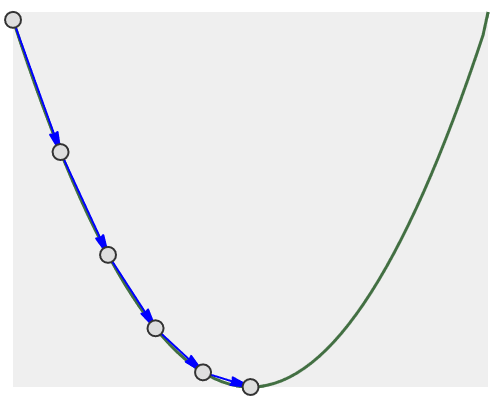
\includegraphics[width=\textwidth]{images/lr_ok.png}
        \caption{Lernrate richtig}
        \label{fig:lr_ok}
    \end{subfigure}
    \begin{subfigure}[b]{0.3\textwidth}
        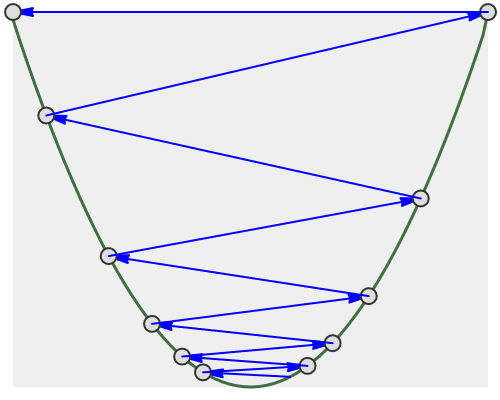
\includegraphics[width=\textwidth]{images/lr_too_high.png}
        \caption{Lernrate zu hoch}
        \label{fig:lr_too_high}
    \end{subfigure}
    \begin{subfigure}[b]{0.3\textwidth}
        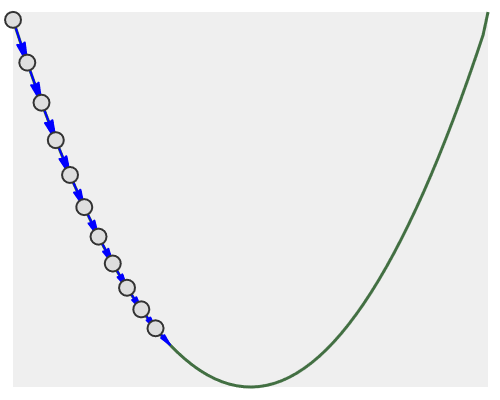
\includegraphics[width=\textwidth]{images/lr_too_low.png}
        \caption{Lernrate zu niedrig}
        \label{fig:lr_too-low}
    \end{subfigure}
    \caption[Lernrate]{Wenn die Lernrate richtig ist, nähert sich der Wert der Verlustfunktion in einer akzeptablen Anzahl von Schritten einem lokalen Optimum an.
    Ist er zu hoch, divergiert er.
    Ist die Lernrate zu niedrig, konvergieren die Werte, aber es sind zu viele Schritte nötig, um dies zu erreichen.
    Bitte beachten Sie, dass diese Bilder den Parameterraum sehr vereinfacht darstellen, da die dargestellte Funktion vollständig konvex und nur zweidimensional ist.}
    \label{fig:learning_rate}
\end{figure}

\subsubsection{Momentum}

Eingeführt 1964 von Polyak \cite{Polyak1964} wird Momentum genutzt, um den Gradienten über mehrere Stufen hinweg konstant zu halten.
Das Momentum bekommt seinen Namen durch eine Analogie zum physikalischen Effekt, nach dem zweiten Newtonschen Bewegungsgesetz \cite[S.12]{Newton1687}.
Die Richtung des Gradienten sollte über mehrere Schritte konsistent sein, und es wäre merkwürdig, wenn die Richtung während des Trainings plötzliche Sprünge macht.
Dies ist nützlich, wenn die Daten "noisy" sind oder einige der Trainingsbeispiele falsch sind, da ihr negativer Effekt durch das Momentum entgegengewirkt wird.
Daher wird ein weiterer Parameter $\nu$ in die Gleichung~\eqref{eq:backprop_update} eingeführt:

\begin{equation}
    \begin{split}
        \nu_{i} &:= \alpha \nu_{i-1} - \eta \varDelta \\
        \theta_{i+1} &:= \theta_i + \nu_i
    \end{split}
    \label{eq:momentum}
\end{equation}

Dagegen ist $\alpha$ ein weiterer Parameter, der eingestellt werden kann, um den Einfluss von $\eta$ auf die Parameter der nächsten Iteration zu regulieren.
Wenn also ein Trainingsbeispiel die "Richtung" des nächsten Schrittes mit einer hohen Abweichung vom Median der letzten Schritte ändern würde, würde die Auswirkung reduziert und die Konvergenzrate möglicherweise verbessert.

Im Jahr 2013 führten Sutskever, Martens, Dahl und Hinton \cite{Sutskever2013} eine weitere Variante des Momentums ein, die von Nesterovs Accelerated Gradient \cite{Nesterov1983} inspiriert wurde.
Diese Variante aktualisiert die zuvor diskutierte Gleichung, um den Parameter zur Berechnung von $\varDelta$ unter Verwendung von $\nu$ zu ändern.
Bitte beachten Sie, dass $\varDelta$ in Gleichung~\eqref{eq:momentum} und ~\eqref{eq:backprop_update} selbst eine Funktion des Parameters $\theta$ ist (siehe Gleichung~\eqref{eq:hidden_error}).

\begin{equation}
    \begin{split}
    \nu_i & := \alpha \nu_i - \eta \varDelta(\theta_i + \alpha \nu_i) \\
    \theta_{i+1} & := \theta_i + \nu_i
    \end{split}
    \label{eq:nesterov}
\end{equation}

Die Idee des Momentums ist, dass der Richtungsvektor in die richtige Richtung zeigt, wobei die Verwendung des Nesterov-Beschleunigten Gradienten wahrscheinlich genauer ist, wenn man mit der Messung des nächsten Fehlers beginnt, der leicht in die jeweilige Richtung verschoben ist \cite[S.353]{Geron2019} \cite[S.291]{Goodfellow2017}.

\subsubsection{Das tatsächliche Training}

Nachdem der Optimierer definiert ist, wird das Modell durch den Aufruf der Modellkompilierfunktion kompiliert.

\begin{lstlisting}
    model.compile(
        loss='sparse_categorical_crossentropy', 
        optimizer=optimizer,
        metrics=['acc'])
\end{lstlisting}

\code{sparse\_categorical\_crossentropy} wird als Verlustfunktion verwendet, wie es für Mehrklassen-Kategorisierungsprobleme empfohlen wird, die durch ganze Zahlen \cite[S.84]{Chollet2017} gekennzeichnet sind.
Sie misst den Abstand zweier Wahrscheinlichkeitsverteilungen, die durch die letzte Schicht des Modells, gegeben durch eine \code{softmax} Aktivierung und die beschrifteten Daten, gegeben sind.
Die SoftMax-Aktivierung wird zur Normalisierung der Ausgabe verwendet, indem jeder Wert durch die Summe aller Werte in der jeweiligen Schicht geteilt wird.
Dies ist nützlich, weil die beschrifteten Daten dem richtigen Knoten den Wert eins und allen anderen den Wert null zuweisen, wodurch sie numerisch vergleichbar werden und dadurch der Verlust für ein sinnvolles Ergebnis minimiert werden kann.

Das eigentliche Training erfolgt dann durch eine \code{Fit}-Funktion im Modell.
Die Trainingsdaten werden durch Generatoren bereitgestellt; die Funktion ist in diesem Fall \code{fit\_generator}.
Daher wird das Training durch den Aufruf der folgenden Funktion durchgeführt:

\begin{lstlisting}
    history = model.fit_generator(
        train_generator,
        steps_per_epoch=20,
        epochs=20,
        callbacks=callbacks)
\end{lstlisting}

Hier wird definiert, dass bei jeder Iteration 20 Bilder als Batch in das Modell eingespeist werden, was für 20 Epochen wiederholt wird.
Nach jeder Epoche aktualisiert der Optimierer die Parameter (die $\theta$ des Modells), was in diesem Durchlauf entsprechend 20 Mal geschieht.

\subsubsection{Results}
\begin{figure}
    \centering
    \begin{subfigure}[b]{0.4\textwidth}
        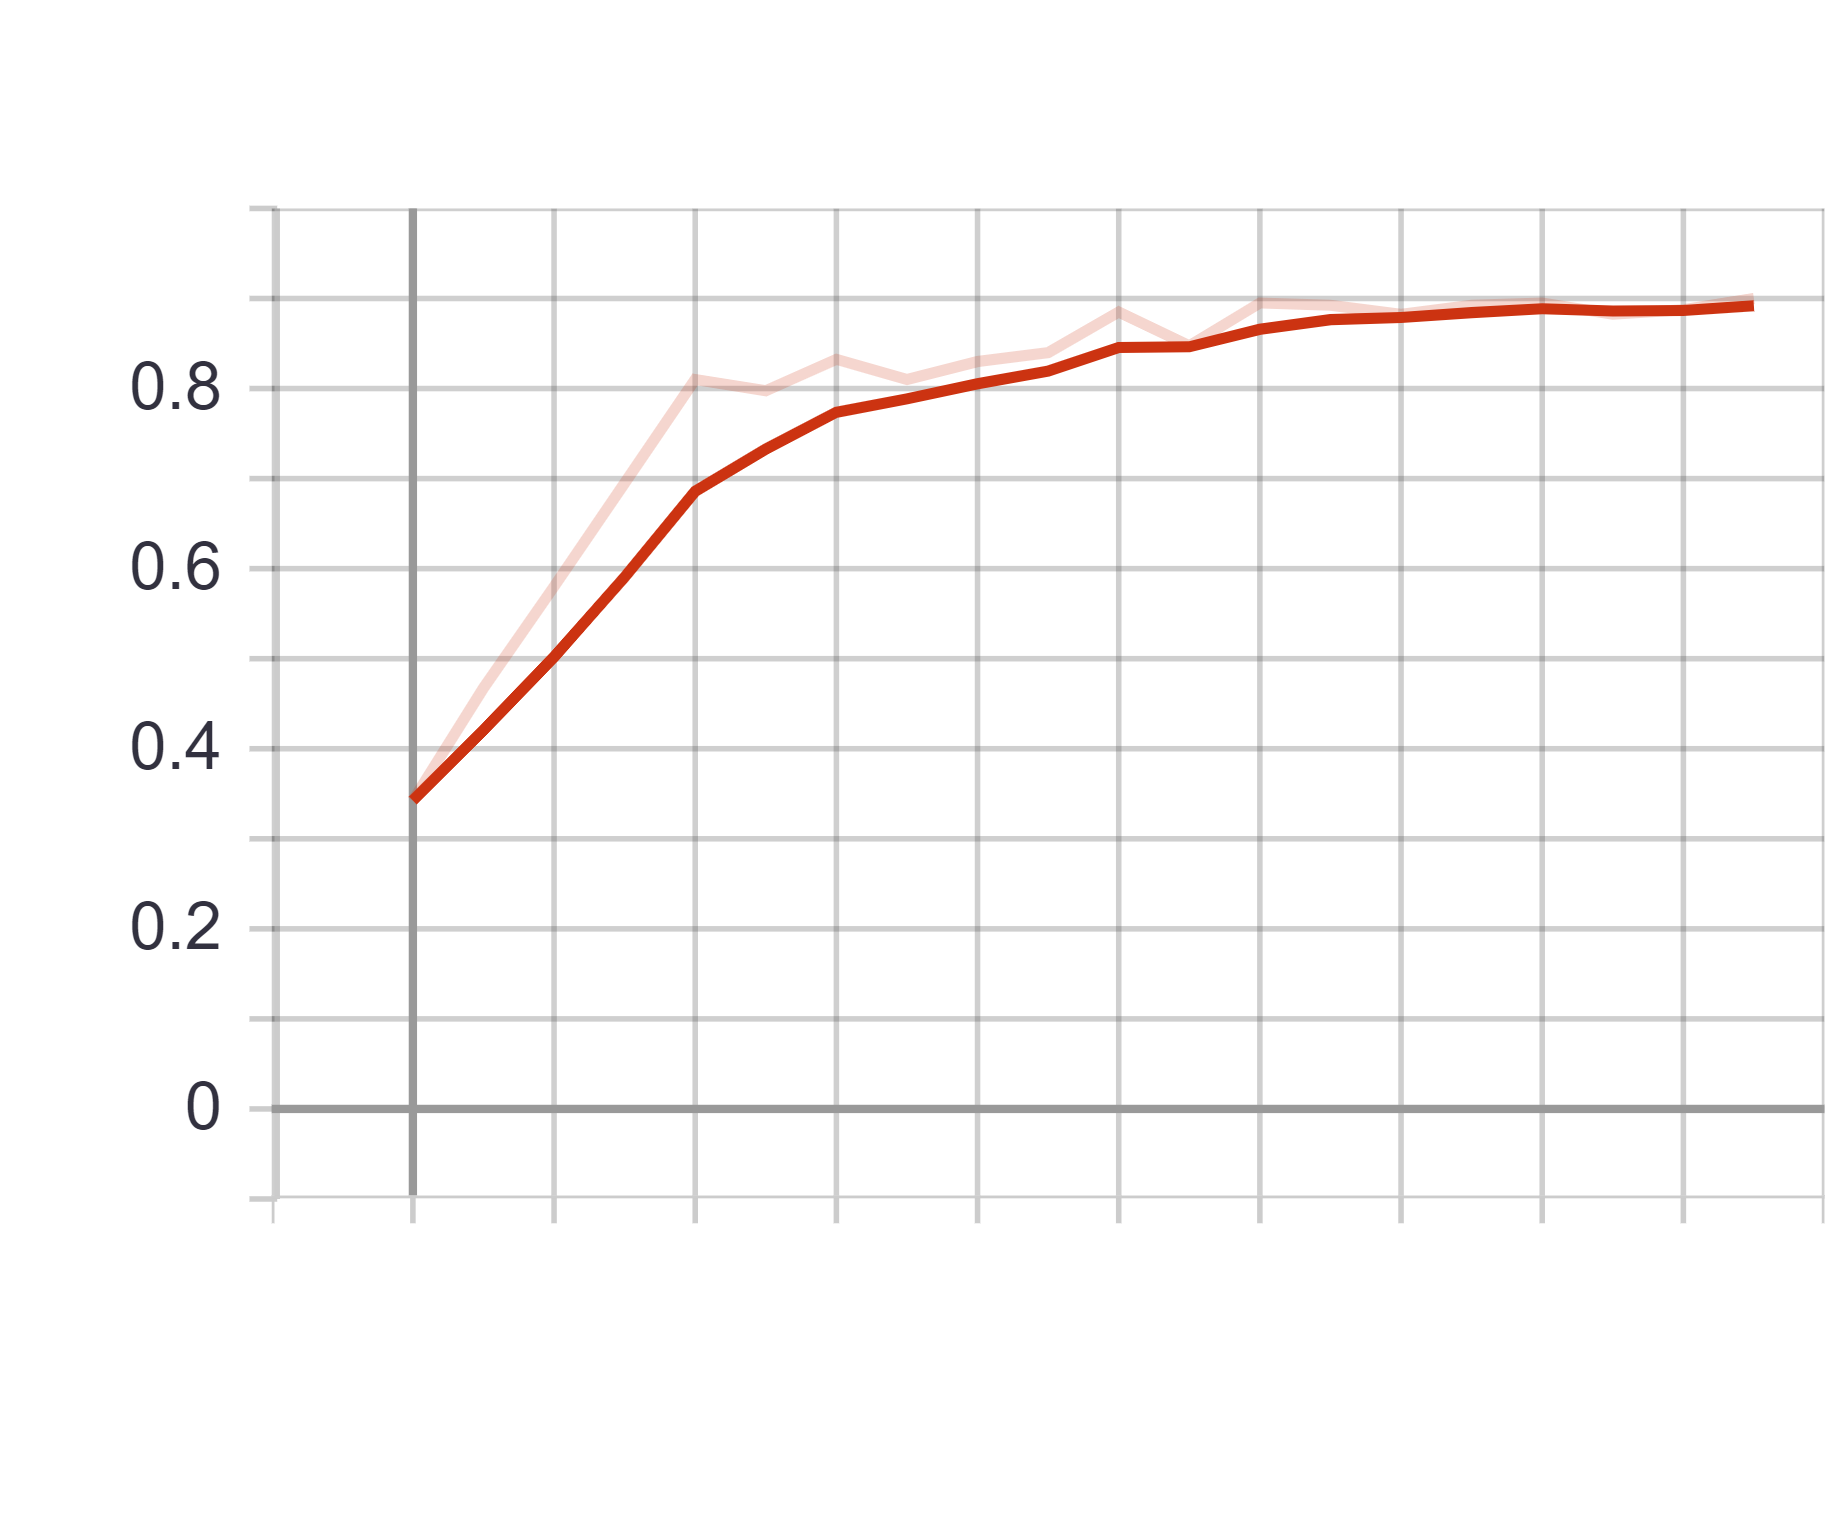
\includegraphics[width=\textwidth]{images/first_model_acc.png}
        \caption{Accuracy}
        \label{fig:first_model_acc}
    \end{subfigure}
    \begin{subfigure}[b]{0.4\textwidth}
        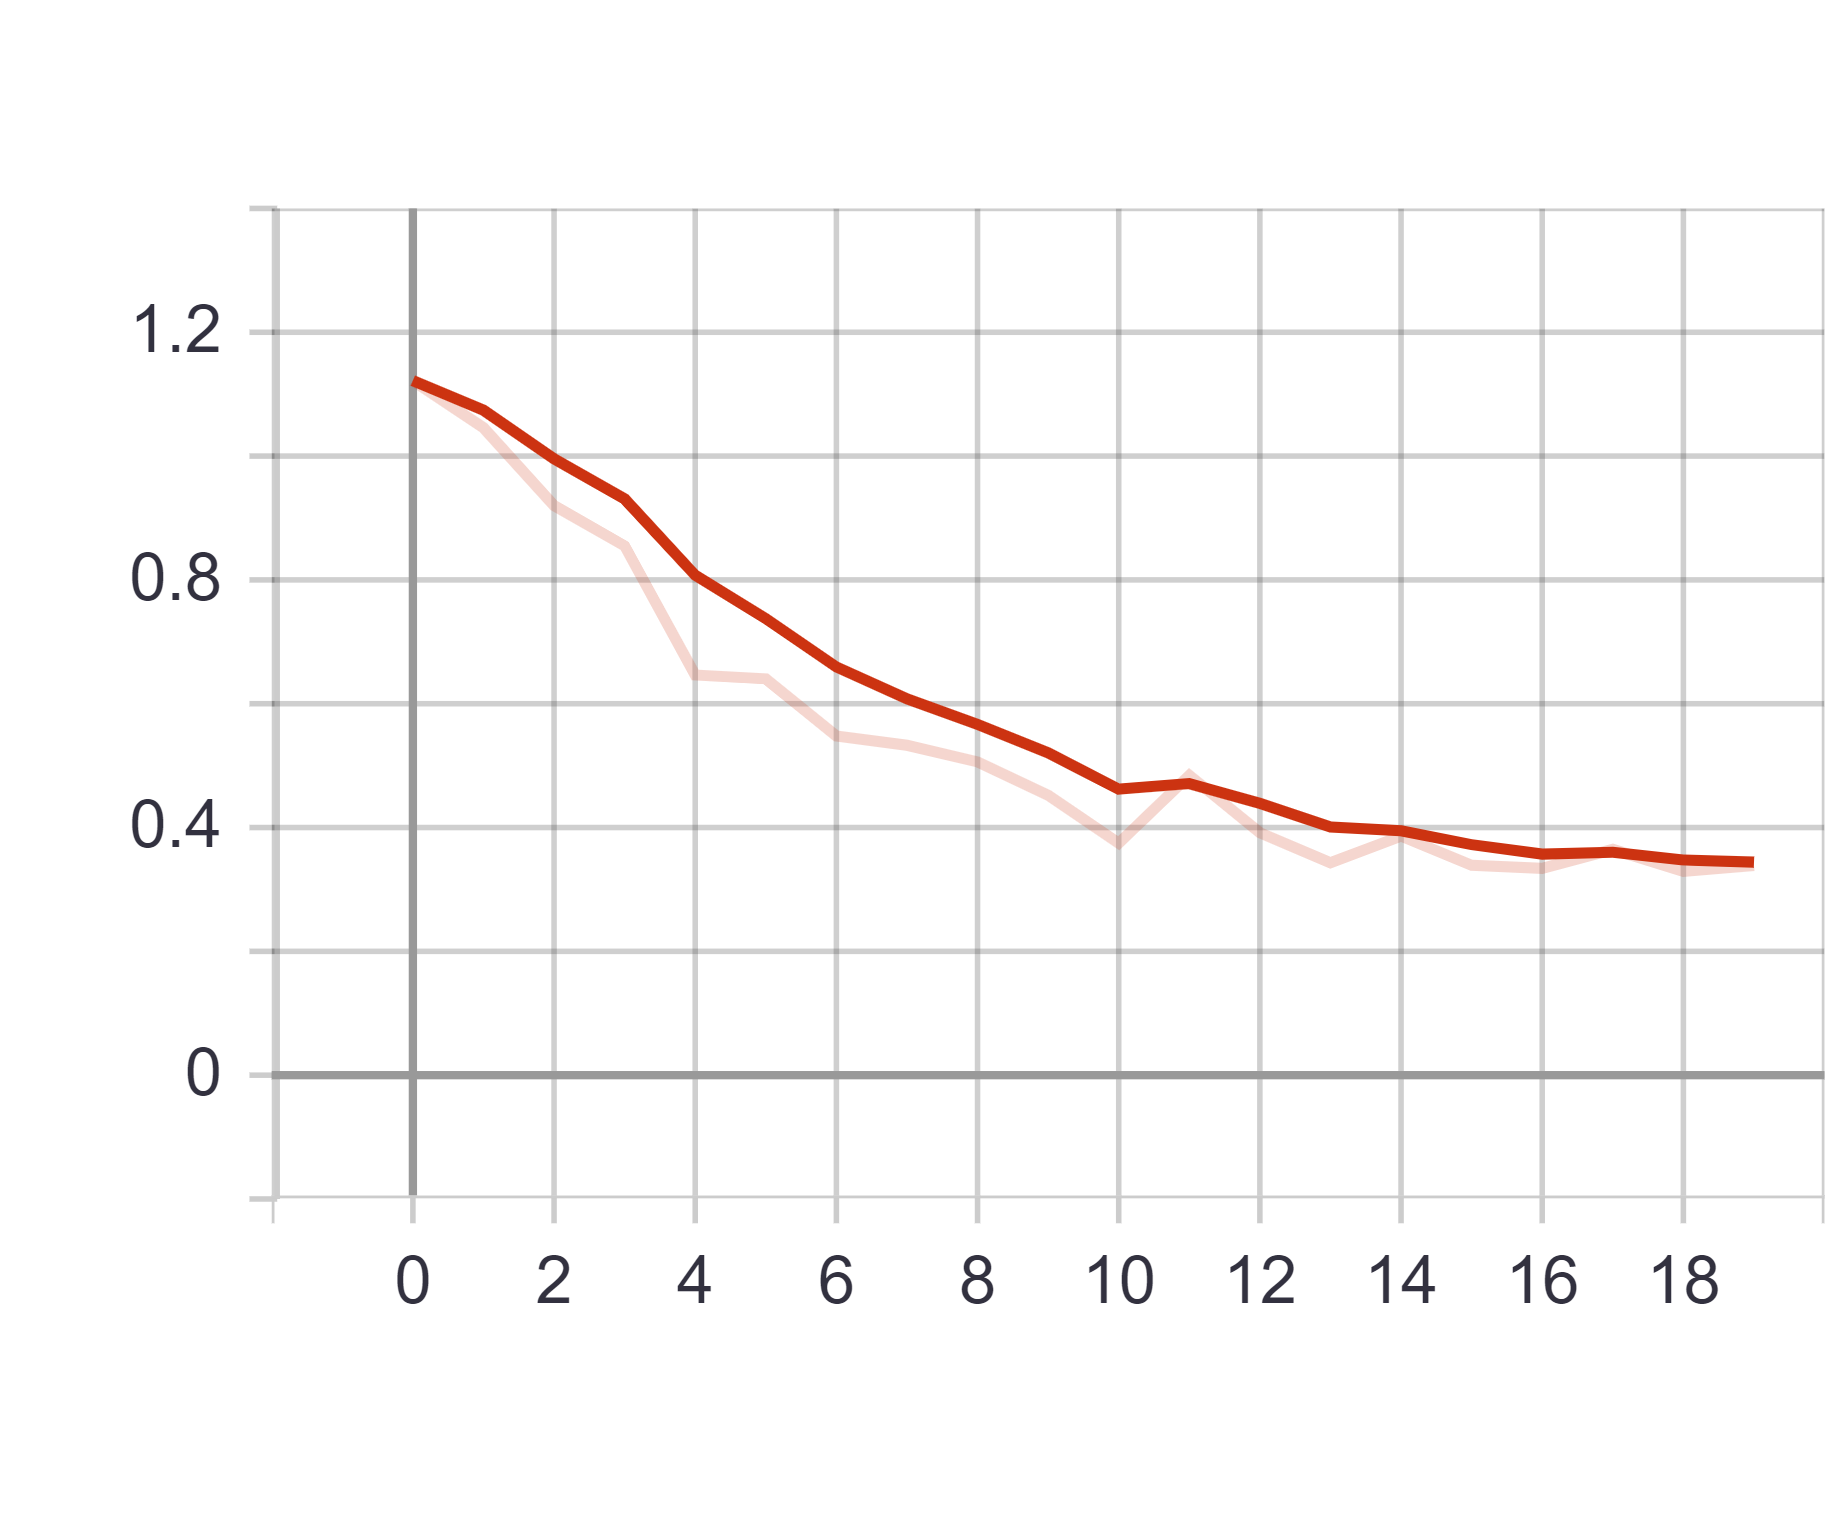
\includegraphics[width=\textwidth]{images/first_model_loss.png}
        \caption{Loss}
        \label{fig:first_model_loss}
    \end{subfigure}
    \caption[Training des ersten Modells]{Die "callbacks" des Trainingsalgorithmus liefern Logs, die von TensorBoard verwendet werden können, um nützliche Grafiken zur Bewertung des Modells bereitzustellen. Die vertikale Achse stellt den Wert der jeweiligen Epoche dar (auf der horizontalen Achse dargestellt).}
    \label{fig:first_model_graphs}
\end{figure}

Wie erwartet, beginnt das Modell mit einer Genauigkeit von etwa 33\%, indem es versucht, die Trainingsdaten in drei Klassen zu klassifizieren.
Wie die Daten nahelegen, lernt das Modell schnell einige Beziehungen zwischen den Eingabedaten und dem jeweiligen Label, da es bereits nach nur vier Epochen eine Genauigkeit von fast 70\% hat.

\begin{lstlisting}
    Epoch 1/20
    20/20 [=====...=====] - 2s 79ms/step - loss: 1.1220 - acc: 0.3425
    Epoch 2/20
    20/20 [=====...=====] - 1s 55ms/step - loss: 1.0457 - acc: 0.4675
    Epoch 3/20
    20/20 [=====...=====] - 1s 55ms/step - loss: 0.9199 - acc: 0.5800
    Epoch 4/20
    20/20 [=====...=====] - 1s 46ms/step - loss: 0.8548 - acc: 0.6950
    ...
    Epoch 17/20
    20/20 [=====...=====] - 1s 45ms/step - loss: 0.3340 - acc: 0.8950
    Epoch 18/20
    20/20 [=====...=====] - 1s 48ms/step - loss: 0.3648 - acc: 0.8825
    Epoch 19/20
    20/20 [=====...=====] - 1s 52ms/step - loss: 0.3291 - acc: 0.8875
    Epoch 20/20
    20/20 [=====...=====] - 1s 47ms/step - loss: 0.3388 - acc: 0.9000
\end{lstlisting}

Nach 20 Epochen hat das Modell eine Genauigkeit von etwa 90\%, was bereits ein sehr guter Anfang für ein erstes Modell mit nicht optimierten Hyperparametern ist.
Wichtig für ein funktionierendes Modell ist, wie gut das Modell Daten klassifiziert, die es noch nie zuvor gesehen hat.
Um dies zu überprüfen, wird ein zweiter Generator erstellt: der \code{test\_generator}, der zur Auswertung des Modells verwendet wird.
Durch die Ausgabe von \code{model.evaluate\_generator(test\_generator)} erhalten wir \code{[0.6071663084129493, 0.7866667]}, der anzeigt, dass der Verlust bei \code{0.60} liegt, im Gegensatz zu \code{0.33} bei den Trainingsdaten und hat und eine Genauigkeit von 78\% bei den Daten noch nie gesehen hat.

Dieses Ergebnis ist ziemlich bemerkenswert, aber offensichtlich schneidet das Modell bei neuen Daten schlechter ab, was darauf hindeutet, dass es bei den Trainingsdaten "overfitted".
Ungeachtet dessen zeigt das Ergebnis, dass durch die Anpassung der Hyperparameter das Ergebnis auf ein zufriedenstellendes Niveau gesteigert werden kann.

Nachdem das Modell trainiert wurde, wird es in \name{models/symbol\_classifier/first\_model.h5} gespeichert und kann zur weiteren Überprüfung in Keras geladen werden.
